% !TeX spellcheck = en_GB

\begin{frame}{Data Science \& Big Data \footnote{Courtesy Prof. F. Transchel, Harz University of Applied Sciences.}}
	\begin{columns}
		
		\begin{column}{0.75\textwidth}
			\begin{tcolorbox}[enhanced jigsaw, colback=white, opacityback=.4, colframe=ElixirPurple, arc=3mm, boxrule=0mm, height=0.75\textheight, valign=center, title=DS Perspective]
					\begin{figure}[htbp]
					\centering
					\resizebox{0.93\columnwidth}{!}{% !TeX spellcheck = en_GB

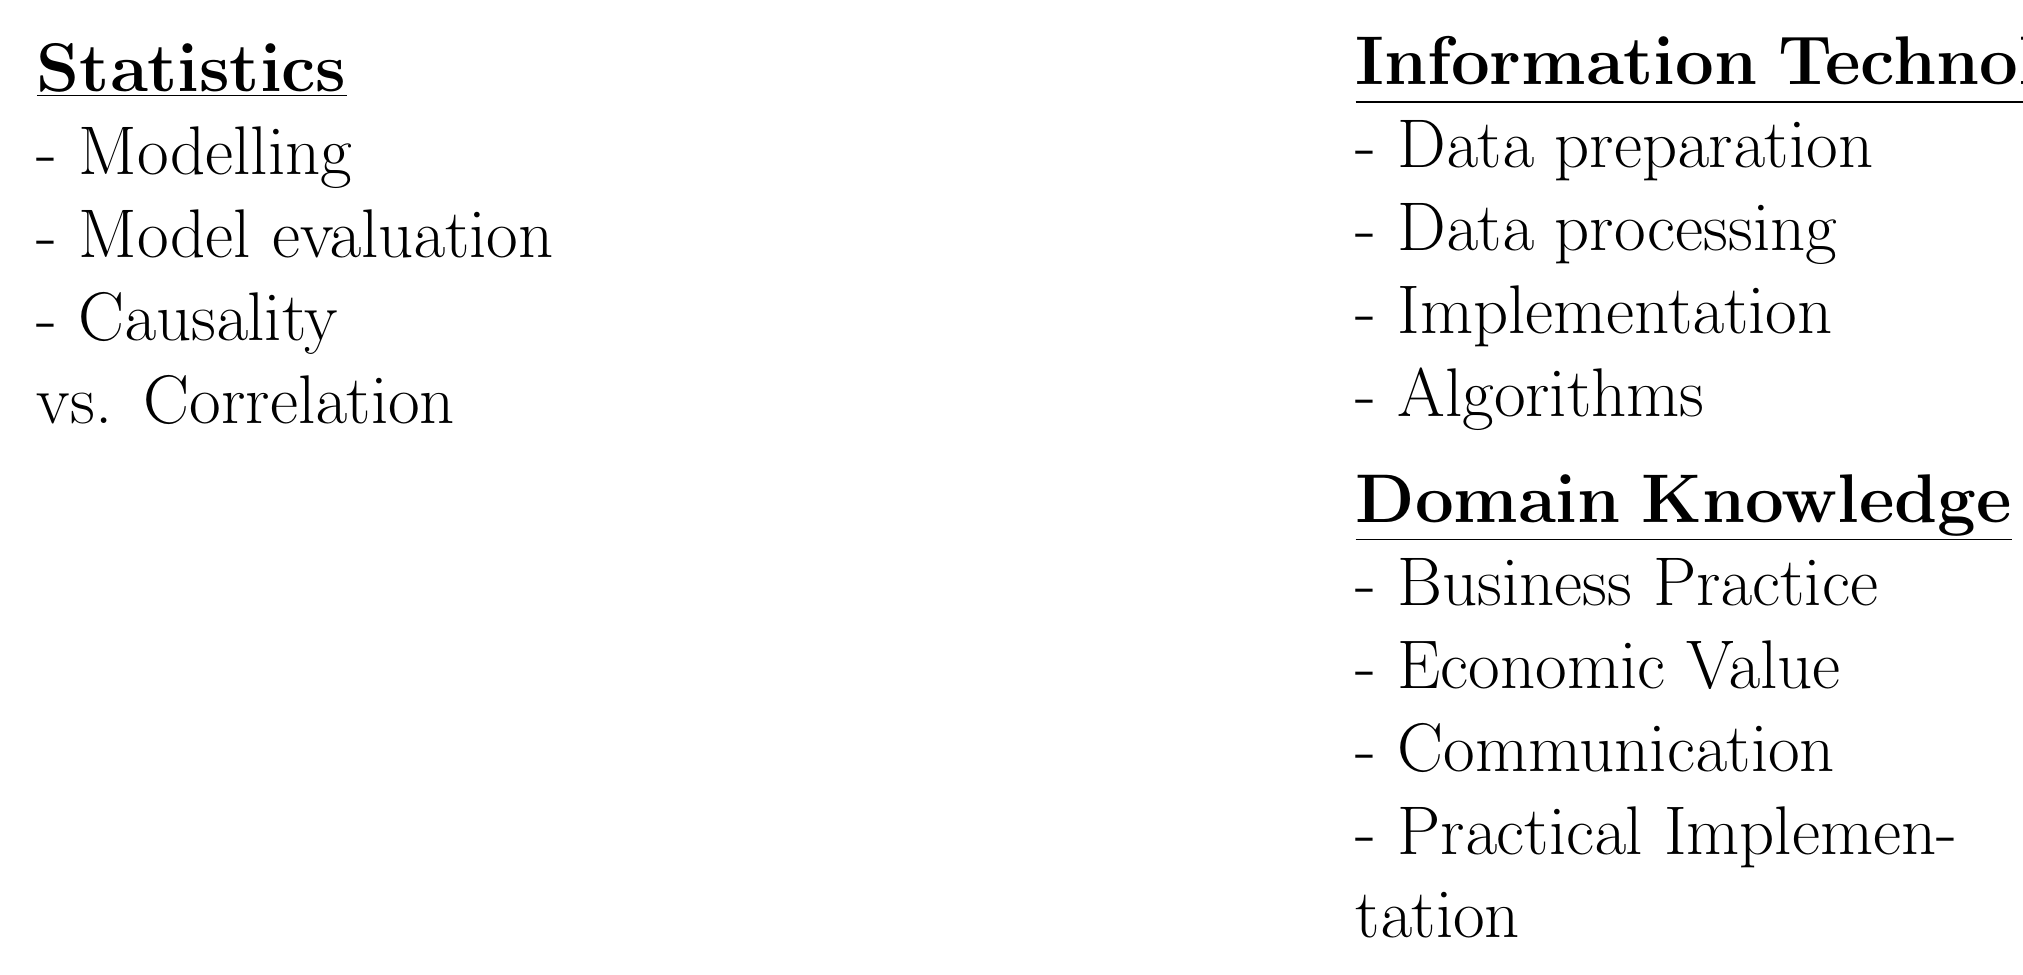
\begin{tikzpicture}[every node/.style={font=\Huge}]

	% Draw the pie chart with separated slices
	\pie[explode=0.3, text=inside, radius=4.5, hide number]{
		33.3/Information \\ Technology,
		33.3/Statistics,
		33.3/Domain \\ Knowledge
	}
	
	% Add legends or annotations
	\node[align=left, anchor=west, text width=7cm] at (5, 3) {
		\underline{\textbf{Information Technology}}\\
		- Data preparation\\
		- Data processing\\
		- Implementation\\
		- Algorithms
	};
	
	\node[align=left, anchor=east, text width=8cm] at (-3.5, 3) {
		\underline{\textbf{Statistics}}\\
		- Modelling\\
		- Model evaluation\\
		- Causality \\ vs. Correlation
	};
	
	\node[align=left, anchor=west, text width=8cm] at (5, -3) {
		\underline{\textbf{Domain Knowledge}}\\
		- Business Practice\\
		- Economic Value\\
		- Communication\\
		- Practical Implementation
	};
\end{tikzpicture}}
					\caption{High Level}
				\end{figure}
			\end{tcolorbox}
		\end{column}
		
		\begin{column}{0.25\textwidth}
			\begin{tcolorbox}[enhanced jigsaw, colback=white, opacityback=.4, colframe=ElixirPurple, arc=3mm, boxrule=0mm, height=0.75\textheight, valign=center, title=Big Data]
				
				\begin{itemize}
					\item Volume
					\item Velocity
					\item Variety
					\vspace{3pt}
					\item Veracity
					\vspace{3pt}
					\item Value
					\item Validity
					
				\end{itemize}
				
			\end{tcolorbox}
		\end{column}
	\end{columns}
\end{frame}

\begin{frame}{CRISP-DM}
	\begin{figure}[htbp]
		\centering
		\resizebox{\columnwidth}{!}{% !TeX spellcheck = en_GB

\definecolor{walnut}{RGB}{61, 43, 31}  % Deep, dark brown color akin to walnut

\tikzset{
	block/.style={
		rectangle,
		draw,
		fill=yellow!30,
		text width=7em,
		text centered,
		rounded corners=3mm,
		minimum height=4em,
		line width=0.7mm,
	},
	arrow/.style={
		thick,
		-{Latex[length=3mm,width=3mm]},
		line width=1mm,
		walnut % Adjusted color
	},
	doublearrow/.style={
		thick,
		{Latex[length=3mm,width=3mm]}-{Latex[length=3mm,width=3mm]},
		line width=1mm,
		walnut % Adjusted color
	},
	decision/.style={
		diamond,
		draw,
		fill=blue!20,
		text width=4.5em,
		text badly centered,
		node distance=3cm,
		inner sep=0pt,
		thick
	},
	dashedarrow/.style={ % Style for dashed arrow
		thick,
		-{Latex[length=3mm,width=3mm]},
		line width=1mm,
		walnut, % Adjusted color
		dashed
	}
}

\begin{tikzpicture}[node distance=1.2cm and 3.5cm]
	% Place nodes
	\node [block] (business) {Business understanding};
	\node [block, right=4.5cm of business] (dataund) {Data understanding};
	\node [block, right=3.0cm of dataund] (dataprep) {Data preparation};
	\node [block, below=of dataprep] (modeling) {Modelling};
	\node [block, below=of dataund] (evaluation) {Evaluation};
	\node [block, below=of business, align=center] (implementation) {Implementation\\into production};
	
	% Draw edges
	\draw [arrow] (dataund) -- (dataprep);
	\draw [doublearrow] (dataprep) -- (modeling); % Arrow starts from the center of the node
	\draw [arrow] (modeling) -- (evaluation);
	\draw [arrow] (evaluation) -- (implementation); % Arrow with head on both ends

	\draw [doublearrow] (business) -- (dataund); % Arrow with head on both ends
	\draw [dashedarrow] (evaluation) -- (business);
	
	% Source text, aligned with the 'Business understanding' node
	\node[anchor=north west, align=left, text width=15cm, below=of implementation, yshift=1cm, xshift=6cm] (source) {Source: P. Chapman, J. Clinton, R. Kerber, T. Khabaza, T. Reinartz, C. Shearer, R. Wirth (2000); CRISP-DM 1.0 Step-by-step data mining guides};
	
	% Dashed box around the diagram
	\node (box) [draw, dashed, walnut, line width=0.75mm, rounded corners=3mm, fit= (dataprep) (dataund) (modeling) (evaluation) , inner sep=2.0mm] {};
	
\end{tikzpicture}
}
		\caption{CRISP-DM: Cross Industry Standard Process for Data Mining}
	\end{figure}
\end{frame}